%%%%%%%%%%%%%%%%%%%%%%%%%%%%%%%%%%%%%%%%%
% Beamer Presentation
% LaTeX Template
% Version 1.0 (10/11/12)
%
% This template has been downloaded from:
% http://www.LaTeXTemplates.com
%
% License:
% CC BY-NC-SA 3.0 (http://creativecommons.org/licenses/by-nc-sa/3.0/)
%
%%%%%%%%%%%%%%%%%%%%%%%%%%%%%%%%%%%%%%%%%

%%% TODOs
%%
%% Link to
%% - Working/Research Group TRs, SRS, etc.

%----------------------------------------------------------------------------------------
%	PACKAGES AND THEMES
%----------------------------------------------------------------------------------------

\documentclass[usenames,dvipsnames,aspectratio=169,serif]{beamer}
\definecolor{cyanprocess}{rgb}{0.0, 0.72, 0.92}
\usecolortheme[named=cyanprocess]{structure}
\usepackage{xcolor}

\usepackage[T1]{fontenc}
\usepackage{fontawesome5}
\usepackage{concmath}
\usepackage{inconsolata}
\setbeamercolor{background canvas}{bg=}%transparent canvas
\usepackage{nomencl}
\usepackage[numbers]{natbib}

\mode<presentation> {

   % The Beamer class comes with a number of default slide themes
   % which change the colors and layouts of slides. Below this is a list
   % of all the themes, uncomment each in turn to see what they look like.

   %\usetheme{default}
   %\usetheme{AnnArbor}
   %\usetheme{Antibes}
   %\usetheme{Bergen}
   %\usetheme{Berkeley}
   %\usetheme{Berlin}
   %\usetheme{Boadilla}
   %\usetheme{CambridgeUS}
   %\usetheme{Copenhagen}
   %\usetheme{Darmstadt}
   %\usetheme{Dresden}
   %\usetheme{Frankfurt}
   %\usetheme{Goettingen}
   %\usetheme{Hannover}
   %\usetheme{Ilmenau}
   %\usetheme{JuanLesPins}
   %\usetheme{Luebeck}
   %\usetheme{Madrid}
   %\usetheme{Malmoe}
   %\usetheme{Marburg}
   %\usetheme{Montpellier}
   %\usetheme{PaloAlto}
   %\usetheme{Pittsburgh}
   %\usetheme{Rochester}
   %\usetheme{Singapore}
   %\usetheme{Szeged}
   \usetheme{Warsaw}

   % As well as themes, the Beamer class has a number of color themes
   % for any slide theme. Uncomment each of these in turn to see how it
   % changes the colors of your current slide theme.

   %\usecolortheme{albatross}
   %\usecolortheme{beaver}
   %\usecolortheme{beetle}
   %\usecolortheme{crane}
   %\usecolortheme{dolphin}
   %\usecolortheme{dove}
   %\usecolortheme{fly}
   %\usecolortheme{lily}
   %\usecolortheme{orchid}
   %\usecolortheme{rose}
   %\usecolortheme{seagull}
   %\usecolortheme{seahorse}
   %\usecolortheme{whale}
   %\usecolortheme{wolverine}

   %\setbeamertemplate{footline} % To remove the footer line in all slides uncomment this line
   %\setbeamertemplate{footline}[page number] % To replace the footer line in all slides with a simple slide count uncomment this line

   %\setbeamertemplate{navigation symbols}{} % To remove the navigation symbols from the bottom of all slides uncomment this line
   %\setbeamertemplate{frametitle}[default][colsep=-4bp,shadow=false,rounded=true]
   \setbeamertemplate{title page}[default][colsep=-0bp,rounded=true]
   \setbeamertemplate{blocks}[rounded][shadow=false]
   \setbeamertemplate{headline}[shadow=false]
   \setbeamertemplate{subsection in head}[shadow=false]
   \setbeamertemplate{section in head}[shadow=false]
   \setbeamertemplate{beamercolorbox}[shadow=false]

}
% \useoutertheme{smoothbars}
%
%
% \makeatletter
% \AtBeginDocument{
% \pgfdeclareverticalshading{beamer@barshade}{\the\paperwidth}{%
%          color(0ex)=(black);%
%          color(0.5ex)=(section in head/foot.bg);%
%          color(4ex)=(section in head/foot.bg)%
%        }
% }
% \makeatother


\usepackage{graphicx} % Allows including images
\usepackage{booktabs} % Allows the use of \toprule, \midrule and \bottomrule in tables

%\usepackage[unicode=true,
% bookmarks=true,bookmarksnumbered=true,bookmarksopen=true,bookmarksopenlevel=1,
% breaklinks=false,pdfborder={0 0 0},pdfborderstyle={},backref=false,colorlinks=true]
% {hyperref}
\hypersetup{
   urlcolor=cyanprocess,
   linkcolor=cyanprocess,
   filecolor=cyanprocess,
   citecolor=cyanprocess,
   pdftitle={Unmanned Traffic Management and Standardisation},
   pdfauthor={Sayandeep Purkayasth},
   pdfsubject={Unmanned Aviation},
   pdfkeywords={Unmanned Aircraft Systems, Unmanned Traffic Management, Standardisation},
}

\usepackage{tikz}
\usetikzlibrary{mindmap,trees,backgrounds}
\usetikzlibrary{shapes,arrows}
\usepackage{xypic}
\xyoption{curve}

%----------------------------------------------------------------------------------------
%	TITLE PAGE
%----------------------------------------------------------------------------------------

\title[UTM \& Stdn.]{Unmanned Traffic Management and Standardisation} % The short title appears at the bottom of every slide, the full title is only on the title page

\author{Sayandeep Purkayasth, PhD} % Your name
\institute[UAWGs] % Your institution as it will appear on the bottom of every slide, may be shorthand to save space
{
   \href{mailto:sayandeep@deepcyan.ai}{sayandeep@deepcyan.ai}  \\ % Your email address
   \medskip
   Unmanned Aviation Working Groups
   \footnote{\tiny \faLink \, https://groups.google.com/forum/\#!forum/utm-wg} % Your email address
   \footnote{\tiny \faEnvelope[regular] utm-wg@googlegroups.com} % Your email address
   \footnote{\tiny \faGit \, https://github.com/utm-working-group} % Your email address
}
\date{7 Nov 2020} % Date, can be changed to a custom date

\begin{document}

\begin{frame}
   \titlepage % Print the title page as the first slide
\end{frame}

\begin{frame}
   \frametitle{Overview} % Table of contents slide, comment this block out to remove it
   \tableofcontents % Throughout your presentation, if you choose to use \section{} and \subsection{} commands, these will automatically be printed on this slide as an overview of your presentation
\end{frame}

%----------------------------------------------------------------------------------------
%	PRESENTATION SLIDES
%----------------------------------------------------------------------------------------

%------------------------------------------------
\section{Introduction} % Sections can be created in order to organize your presentation into discrete blocks, all sections and subsections are automatically printed in the table of contents as an overview of the talk
%------------------------------------------------

\subsection{UA Working Groups} % A subsection can be created just before a set of slides with a common theme to further break down your presentation into chunks

\begin{frame}
   \frametitle{UA Working Groups}
   \begin{figure}[tbh]
      \begin{centering}
         \begin{center}
            \small\tt
            \hfil
            \xymatrix{
               %& \txt{DFI} \ar[dr] & \txt{MoCA} \ar[d] & \cdots \ar[dl] & \\
               % & & \txt{UA Society} \ar[d] & & \\
               % & & \txt{Steering \\Committee} \ar[dl] \ar[dr] & & \\
               & & \txt{Working Groups} \ar@{-}@/_/[dll] \ar@{-}[dl] \ar@{-}[d] & \txt{Research Groups} \ar@{-}[d] \ar@{-}[dr] & \\
               *+{\txt{NPNT}} & *+[F--]{\txt{Remote ID}} & *+[F]{\txt{UTM}} & *+{\txt{Risk}} & *+{\txt{Deconfliction}} }
         \hfil \end{center}
      \par\end{centering}
      \caption{Unmanned Aviation Working and Research Groups}
   \end{figure}
\end{frame}

%------------------------------------------------

\begin{frame}
   \frametitle{UA Working Groups}
   \framesubtitle{Members}
   \begin{table}\small\ttfamily
      \begin{tabular}{ l | l | l }
         iSpirt & Algopixel Technologies\footnotemark & Deepcyan Software\footnotemark[\value{footnote}] \\
         Skylark Drones\footnotemark[\value{footnote}] & Drone Federation of India\footnotemark[\value{footnote}] & UniFly\footnotemark[\value{footnote}] \\
         IISc & Asteria & HexCod \\
         Curl Analytics & Avianco\footnotemark[\value{footnote}] & IdeaForge \\
         AUS & Omnipresent Tech & IIT Bombay \\
         Drone Aerospace & QTPI & PDRL\footnotemark[\value{footnote}] \\
      \end{tabular}
   \end{table}
   \footnotetext{Opinions expressed in published materials may not represent the views of organisations except as marked.}
\end{frame}

%------------------------------------------------

\subsection{Nomenclature}

\begin{frame}
   \frametitle{Nomenclature}
   \begin{table}\scriptsize\ttfamily
      \begin{tabular}{ l|l }
         UAS & Unmanned Aerial System \\
         RPAS & Remotely Piloted Aircraft System \\
         UTM & Unmanned Traffic Management \\
         USS & UAS Service Supplier \\
         DCSP & Data Collection Service Provider \\
         CAA & Civil Aviation Authority \\
         DGCA & Directorate General of Civil Aviation, GoI \\
         NPNT & No Permission No Takeoff \\
         ATC & Air Traffic Control \\
         UAOP & Unmanned Aircraft Operator Permit \\
         UIN & Unique Identification Number \\
         DSP & DigitalSky\texttrademark \, Service Provider \\
         ANSP & Air Navigation Service Provider \\
      \end{tabular}
   \end{table}
\end{frame}

%------------------------------------------------

\subsection{Overview}

\begin{frame}
   \frametitle{Stakeholders}
   % MIND MAP

   \begin{columns}[c] % the "c" option specifies center vertical alignment
      \begin{column}{.6\textwidth} % column designated by a command
         \begin{tikzpicture}[scale=0.5,transform shape]
            \ttfamily
            \path[mindmap,concept color=cyanprocess,text=white]
            node[concept] {Unmanned Traffic Management}
            [clockwise from=0]
            child [concept color=RoyalBlue!50!cyanprocess] { node[concept] (c3) {UAS} }
            child [concept color=OliveGreen] { node[concept] (c1) {Operator} }
            child [concept color=Maroon] { node[concept] (c2) {Pilot} }
            child [concept color=black] { node[concept] (c5) {Manned Air Traffic Control} }
            child [concept color=YellowOrange] { node[concept] (c4) {Civil Aviation Authority} }
            child [concept color=Violet] { node[concept ] (c0) {Manufacturer} };
            % \begin{pgfonlayer}{background}
            %    \draw [concept connection]  (c1) edge (c2)
            %    edge (c3)
            %    (c2) edge (c3);
            % \end{pgfonlayer}
         \end{tikzpicture}
      \end{column}
      \begin{column}{.4\textwidth}
         Others
         \begin{itemize}
            \item Military
            \item Law Enforcement
            \item Airports
            \item Insurance providers
         \end{itemize}
         See also FAA Concept of Operations \cite{FAA-ConOps-v2}.
      \end{column}
   \end{columns}
\end{frame}

%------------------------------------------------

\begin{frame}
   \frametitle{Need and Expectations}
   See also a survey on UTM systems \cite{ISO-TR-23629-1-2020}.
   \begin{columns}[t]
      \column{.45\textwidth}
      \begin{itemize}
         \item Increasing number of drones, flights, pilots
         \item Standardised communication between UTMs
         \item Communication between stakeholders
         \item Enabling newer use cases
         \item Maintaining operational privacy, safety and security
      \end{itemize}
      \column{.45\textwidth}
      \begin{itemize}
         \item Deconfliction
            \begin{itemize}
               \item Other Unmanned air traffic
               \item Manned air traffic
            \end{itemize}
         \item Regulatory compliance
         \item Supporting safer flight planning
         \item Identification of risk factors for complex operations
         \item Realtime situational awareness and Separation
      \end{itemize}
   \end{columns}
\end{frame}

%------------------------------------------------

\begin{frame}
   \frametitle{UTM}
   \framesubtitle{Architecture}
   \begin{columns}[T]
      \begin{column}{0.6\textwidth}
         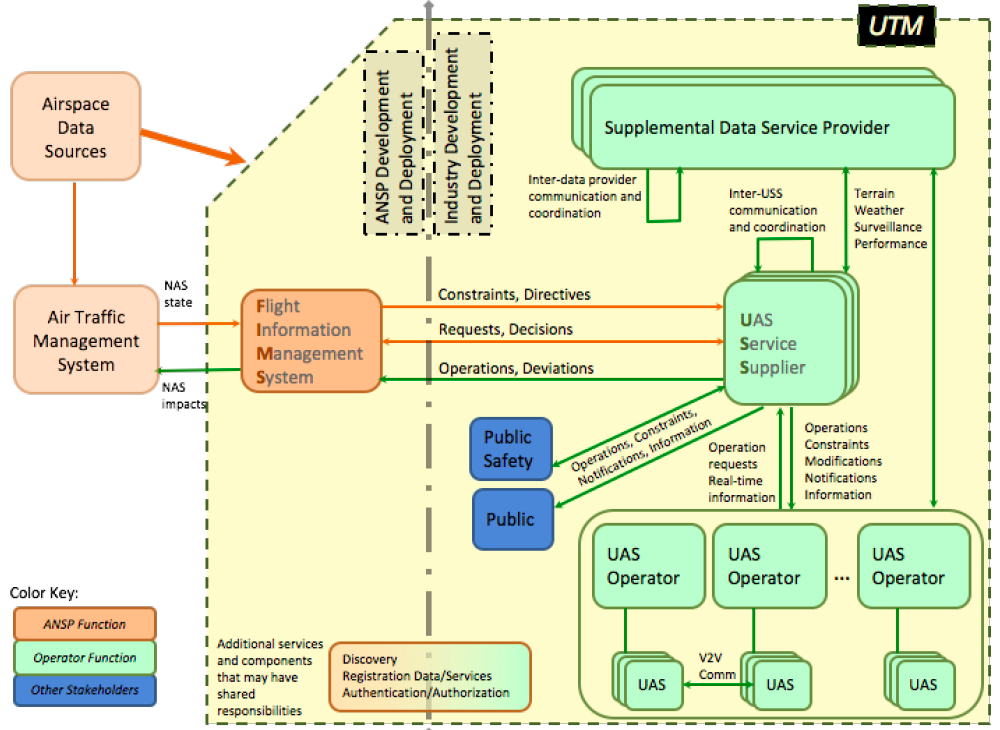
\includegraphics[height=0.75\textheight]{img/utm-architecture.png}
      \end{column}
      \begin{column}{0.4\textwidth}
         JARUS UTM architecture \cite{JARUS-SORA/JAR-DEL-WG6-D.04}
      \end{column}
   \end{columns}

\end{frame}

%------------------------------------------------

\begin{frame}
   \frametitle{Services: CAA Registration}
   For comprehensive service listing and details see UTM SRS (draft) \cite{UTMWG-SRS} and DGCA RPAS Guidance Manual \cite{RPASGM2020} (also referred to as NPNT).
   \begin{block}{UAS}
      UIN Application, UAS Acquisition
   \end{block}

   \begin{block}{Manufacturer}
      Profile Management \& Permission Management
   \end{block}

   \begin{block}{Operator}
      Profile \& Permission Management, UAOP Application
   \end{block}

   \begin{block}{Pilot}
      Profile Management \& Permission Management
   \end{block}
\end{frame}

%------------------------------------------------

\begin{frame}
   \frametitle{Services: Operational}
   \begin{columns}[t] % The "c" option specifies centered vertical alignment while the "t" option is used for top vertical alignment

      \column{.45\textwidth} % Left column and width
      \begin{itemize}
         \item Flight Planning
         \item Flight Awareness
         \item Communication \& Navigation
         \item Dynamic Airspace Density
         \item Weather
      \end{itemize}

      \column{.45\textwidth} % Right column and width
      \begin{itemize}
         \item Log Management
         \item Mapping
         \item Airspace authorisation
         \item Incident Reporting
      \end{itemize}
   \end{columns}
\end{frame}
%------------------------------------------------

\begin{frame}
   \frametitle{Functions: Operational (contd.)}
   \begin{columns}[t] % The "c" option specifies centered vertical alignment while the "t" option is used for top vertical alignment

      \column{.45\textwidth} % Left column and width
      \begin{itemize}
         \item Deconfliction
            \begin{itemize}
               \item Advisory \& Alert
               \item Strategic
               \item Tactical / Dynamic Reroute
            \end{itemize}
         \item Restrictions
      \end{itemize}

      \column{.45\textwidth} % Right column and width
      \begin{itemize}
         \item Conformance Monitoring
         \item Risk reduction
         \item Messaging
         \item Flight Notification
      \end{itemize}
   \end{columns}

\end{frame}

%------------------------------------------------
\section{Services}
%------------------------------------------------

% \subsection{Registration}
% \begin{frame}
%    \frametitle{Registration}
%    \framesubtitle{UAS}
%    \begin{columns}[t]
%       \begin{column}{0.5\textwidth}
%       \end{column}
%       \begin{column}{0.5\textwidth}
%       \end{column}
%    \end{columns}
% \end{frame}
%
% \begin{frame}
%    \frametitle{Registration}
%    \framesubtitle{Manufacturer}
%    \begin{columns}[t]
%       \begin{column}{0.5\textwidth}
%       \end{column}
%       \begin{column}{0.5\textwidth}
%       \end{column}
%    \end{columns}
% \end{frame}
%
% \begin{frame}
%    \frametitle{Registration}
%    \framesubtitle{Operator}
% \end{frame}
%
% \begin{frame}
%    \frametitle{Registration}
%    \framesubtitle{Pilot}
%    \begin{columns}[t]
%       \begin{column}{0.5\textwidth}
%       \end{column}
%       \begin{column}{0.5\textwidth}
%       \end{column}
%    \end{columns}
% \end{frame}
%
%------------------------------------------------

%% FLIGHT PLANNING

\subsection{Operations}
\begin{frame}
   \frametitle{Flight Planning}
   \begin{columns}[T]
      \begin{column}{0.75\textwidth}
         Actor: Pilot/Operator \\
         Stage: Pre-flight \\
         {Objective: Support operator in defining flight geography that meets the needs of their mission while complying with the spatial/temporal boundaries and authorisation constraints} \\
         Input: UAS performance, communication and navigation performance, contingency actions, launch/recovery behavior, etc. The service would also utilize data from other available services (e.g. weather service). \\
         Output: Suggestions on flight path modifications and Flight Geography Volume generated from the flight path
      \end{column}
      \begin{column}{0.25\textwidth}
         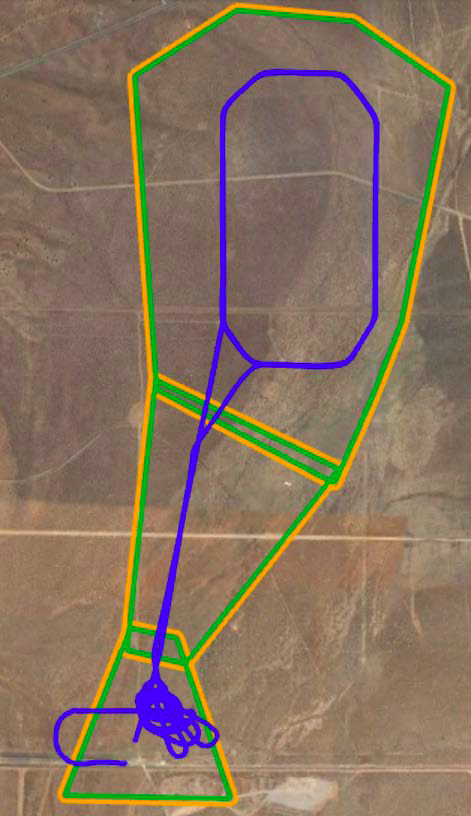
\includegraphics[height=0.75\textheight]{img/flight-planning.png}
      \end{column}
   \end{columns}
\end{frame}

%% FLIGHT AWARENESS

\begin{frame}
   \frametitle{Flight Awareness}
   \begin{columns}[T]
      \begin{column}{0.65\textwidth}
         Actor: Pilot/Operator \\
         Stage: Pre-flight \\
         Related services: Flight Planning \\
         APIs: Pilot $\leftrightarrow$ UTM; UTM $\leftrightarrow$ UTM; UTM $\leftrightarrow$ CAA \\
         Objective: Provides a UAS operator contextual geographic information that supports awareness of areas in which flight operations and/or launch and recover are not permitted.  \\
         Input: Intended Operation volume. The service would consider flight restricted and conditionally restricted areas and notify an operator of the potential hazard or restriction.
      \end{column}
      \begin{column}{0.35\textwidth}
         Output: Notification of existing or future known restrictions that intersect with the operation volume \\
         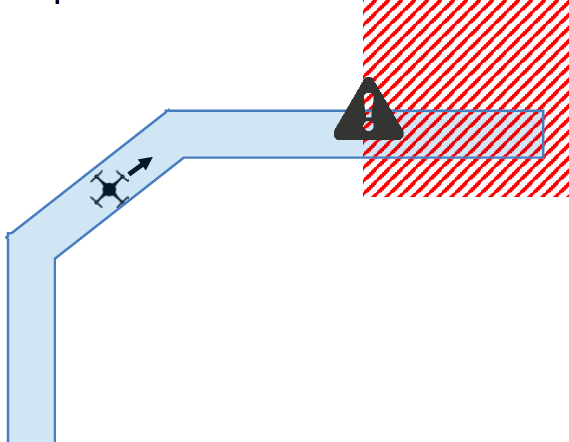
\includegraphics[height=0.65\textwidth]{img/flight-awareness.png}
      \end{column}
   \end{columns}
\end{frame}

\begin{frame}
   \frametitle{Communication \& Navigation}
   \begin{columns}[t]
      \begin{column}{0.5\textwidth}
         Objective: Provide
         \begin{itemize}
            \item historical performance data during for airspace surveying during the safety development phase
            \item coverage maps during the flight planning phase
            \item real-time integrity, availability, quality of service, and security monitoring during the operation phase.
         \end{itemize}
      \end{column}
      \begin{column}{0.5\textwidth}
         Operator Use:
         \begin{itemize}
            \item  Flight Planning: UAS operator would utilize coverage maps to ensure develop flight plans and contingency management procedures are consistent with CAA requirements, UAS performance, and mission objectives.
         \end{itemize}
         Output: Notifications and information associated with the quality of service and performance of the third party communication systems. \\
      \end{column}
   \end{columns}
\end{frame}

\begin{frame}
   \frametitle{Communication \& Navigation (contd.)}
   \begin{columns}[t]
      \begin{column}{0.5\textwidth}
         Operator Use:
         \begin{itemize}
            \item  Real-time Monitoring support using a Communication and Navigation Service would entail the service provider supplying a monitor of the integrity and QoS of the communication network, system and/or navigation solution over a given geographic area.
         \end{itemize}
      \end{column}
      \begin{column}{0.5\textwidth}
         Operator Use:
         \begin{itemize}
            \item Monitors would identify areas of degraded coverage, increased latency, or high probability of interference.
            \item The real-time monitoring capability would also notify the UAS operator of any reported communication blackout or jamming.
         \end{itemize}
      \end{column}
   \end{columns}
\end{frame}

\begin{frame}
   \frametitle{Dynamic Airspace Density \& Log Management}
   \begin{columns}[t]
      \begin{column}{0.5\textwidth}
         \begin{block}{Dynamic Airspace Density}
         Actor: Pilot/Operator \\
         Stage: Pre- or during-flight \\
         Related services: Flight Planning \\
         APIs: Pilot $\leftrightarrow$ UTM; UTM $\leftrightarrow$ CAA \\
         Input: Operational volume (intended or otherwise) \\
         Output: Predicted air traffic density in volume and time restrictions of operation
         \end{block}
      \end{column}
      \begin{column}{0.5\textwidth}
         \begin{block}{Log Management}
         Actor: Pilot/Operator \\
         Stage: Post-flight \\
         APIs: Pilot $\rightarrow$ UTM; UTM $\rightarrow$ CAA \\
         Objective: Provide CAA flight log
         Output: None
         \end{block}
      \end{column}
   \end{columns}
\end{frame}

\begin{frame}
   \frametitle{Incident Reporting \& Restrictions}
   \begin{columns}[t]
      \begin{column}{0.5\textwidth}
         \begin{block}{Incident Reporting}
         Actor: Pilot/Operator \\
         Stage: Post-flight \\
         APIs: Pilot $\rightarrow$ UTM, UTM $\rightarrow$ CAA \\
         Input: Incident Report\\
         Output: None \\
         \end{block}
      \end{column}
      \begin{column}{0.5\textwidth}
         \begin{block}{Restrictions}
         Actor: Pilot/Operator \\
         Stage: Pre-flight \\
         APIs: Pilot $\leftrightarrow$ UTM, UTM $\leftrightarrow$ CAA \\
         Input: Operational volume (intended or otherwise)\\
         Output: Temporary Flight Restrictions (manned) or Volume Restrictions (unmanned)
         \end{block}
      \end{column}
   \end{columns}
\end{frame}

\begin{frame}
   \frametitle{Weather}
   \begin{columns}[t]
      \begin{column}{0.5\textwidth}
         Actor: Pilot/Operator \\
         Stage: Pre-flight \& during-flight \\
         APIs: Pilot $\leftrightarrow$ UTM \\
         Objective: Support UAS Operator's awareness of atmospheric conditions in the geographic area in which they will be conducting operations.
         \begin{itemize}\small
         \item  Near term, short term and long term forecasting of local and regional atmospheric conditions
         \item  User provided hazardous weather reports, known as UAS Reports (UREP).
         \end{itemize}
      \end{column}
      \begin{column}{0.5\textwidth}
         \begin{itemize}\small
         \item  Real-time weather reporting
         \item  Weather advisories and alerts for a given geographic area
         \item  Operation specific weather alerts that highlight areas in the operation volume where weather posses an elevated to risk to mission success and/or safety.
         \item  Interfacing weather information with the Dynamic Rerouting Service to provide dynamic weather routes to avoid hazardous conditions.
         \end{itemize}
      \end{column}
   \end{columns}
\end{frame}

% \begin{frame}
%    \frametitle{Mapping}
%    \begin{columns}[t]
%       \begin{column}{0.5\textwidth}
%          Actor: Pilot/Operator \\
%          Stage: Pre-flight \& during-flight \\
%          APIs: Pilot $\rightarrow$ UTM \\
%       \end{column}
%       \begin{column}{0.5\textwidth}
%          Objective: \\
%          Example output: \\
%       \end{column}
%    \end{columns}
% \end{frame}
%
% \begin{frame}
%    \frametitle{Airspace authorisation}
%    \begin{columns}[t]
%       \begin{column}{0.5\textwidth}
%          Actor: Pilot/Operator \\
%          Stage: Post-flight \\
%          APIs: Pilot $\rightarrow$ UTM, UTM $\rightarrow$ CAA \\
%       \end{column}
%       \begin{column}{0.5\textwidth}
%          Objective: \\
%          Example output: \\
%       \end{column}
%    \end{columns}
% \end{frame}
%
\begin{frame}
   \frametitle{Conformance Monitoring}
   \begin{columns}[t]
      \begin{column}{0.5\textwidth}
         Stage: During-flight \\
         APIs: UAS $\leftrightarrow$ UTM, UTM $\rightarrow$ CAA \\
         Operator Use: Service monitors the UAS position and notifies the UAS Operator if they deviate from the Flight Geography. A conformance threshold is applied between the Flight Geography and Operation Volume (Conformance Volume) and if the UAS crosses the threshold the service provides a traffic advisory to other proximal UAS Operators.
      \end{column}
      \begin{column}{0.5\textwidth}
         Output:
         \begin{itemize}\small
         \item  Notification of deviations
         \item  Notification to other UAS Operators of deviations
         \item  Position sharing to other UAS Operators if deviation occurs
         \end{itemize}
         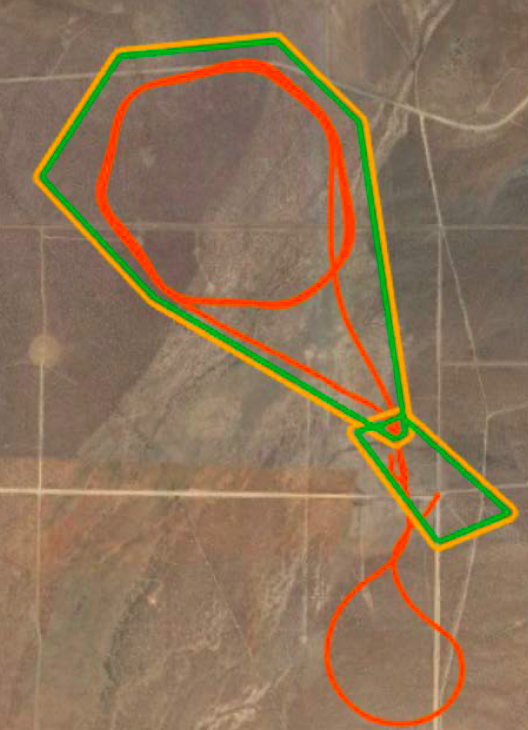
\includegraphics[height=0.45\textwidth]{img/conformance-monitoring.png}

      \end{column}
   \end{columns}
\end{frame}

\begin{frame}
   \frametitle{Risk reduction}
   \begin{columns}[t]
      \begin{column}{0.5\textwidth}
         Actor: Pilot/Operator \\
         Stage: Pre-flight \\
         APIs: Pilot $\leftrightarrow$ UTM, UTM $\rightarrow$ CAA \\
         Input: Operational parameters, volume \\
         Example output: Ground risk, Air risk categories Specific Assurance and Integrity Levels, Known risk factors \\
      \end{column}
      \begin{column}{0.5\textwidth}
         See also: Technical Report on UA Risk Assessment (draft) \cite{UARRG-TR-1}, ATM airspace assessment \cite{EASA-UAS-ATM-Assessment-2018} and JARUS SORA process \cite{JARUS-SORA/JAR-DEL-WG6-D.04}
      \end{column}
   \end{columns}
\end{frame}

% \begin{frame}
%    \frametitle{Messaging}
%    \begin{columns}[t]
%       \begin{column}{0.5\textwidth}
%          Actor: Pilot/Operator \\
%          Stage: Post-flight \\
%          APIs: Pilot $\rightarrow$ UTM, UTM $\rightarrow$ CAA \\
%       \end{column}
%       \begin{column}{0.5\textwidth}
%          Objective: \\
%          Example output: \\
%       \end{column}
%    \end{columns}
% \end{frame}
%
\begin{frame}
   \frametitle{Flight Notification}
   \begin{columns}[t]
      \begin{column}{0.5\textwidth}
         Actor: Pilot/Operator, Any \\
         APIs: Pilot $\leftrightarrow$ UTM, UTM $\leftrightarrow$ CAA \\
         Objective: Disseminate information regarding UAS operations in a given geographic areas to other airspace users, non-UAS stakeholders, local, state, and tribal governments, and the general public. UAS Operator would get an indication of anticipated level of UAS traffic. \\
         Example Service Outputs:
      \end{column}
      \begin{column}{0.5\textwidth}
         \begin{itemize}\small
         \item  Density of operations
         \item  Expected duration at given density levels
         \item  Expected maximum UAS cruise altitudes
         \item  Approximate launch/recovery locations
         \end{itemize}
         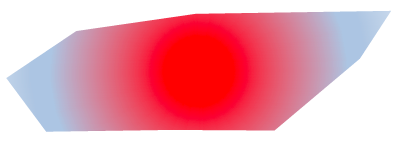
\includegraphics[height=0.35\textwidth]{img/flight-notification.png}
      \end{column}
   \end{columns}
\end{frame}


\subsection{Deconfliction}

\begin{frame}
   \frametitle{Deconfliction}
   \begin{columns}[t]
      \begin{column}{0.25\textwidth}
      \end{column}
      \begin{column}{0.5\textwidth}
         \begin{block}{Conflict}
            Two or more UASs, flight plans or operations are in conflict if they overlap in spatial (latitude, longitude, altitude) and temporal dimensions.
         \end{block}
      \end{column}
      \begin{column}{0.25\textwidth}
      \end{column}
   \end{columns}
\end{frame}

\begin{frame}
   \frametitle{Deconfliction}
   \framesubtitle{Advisory \& Alert}
   \begin{columns}[t]
      \begin{column}{0.5\textwidth}
         Actor: Pilot/Operator \\
         Stage: Pre-flight \\
         Related services: Flight Planning \\
         APIs: Pilot $\leftrightarrow$ UTM; UTM $\leftrightarrow$ UTM; UTM $\leftrightarrow$ CAA \\
         Objective: Supports a UAS operator by providing real-time or in-time data regarding the proximity to potential conflicting aircraft.
      \end{column}
      \begin{column}{0.5\textwidth}
         Output: Informative, suggestive, and directive guidance to support the UAS Operator in conflict resolution \\
         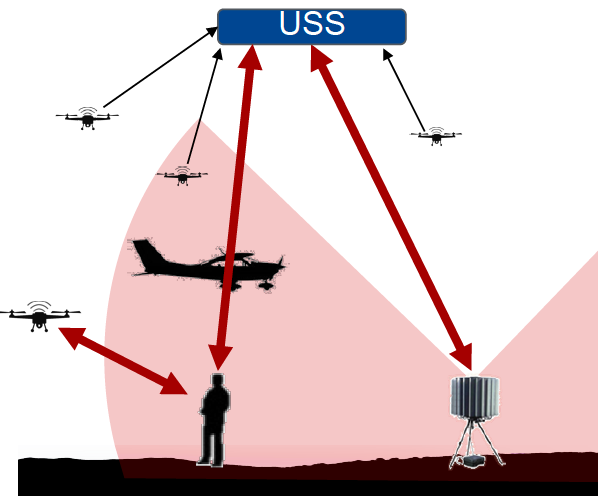
\includegraphics[height=0.45\textwidth]{img/conflict-advisory.png}

      \end{column}
   \end{columns}
\end{frame}

%% 9 STRATEGIC DECONFLICTION

\begin{frame}
   \frametitle{Deconfliction}
   \framesubtitle{Strategic}
   \begin{columns}[t]
      \begin{column}{0.5\textwidth}
         Actor: Pilot/Operator \\
         Stage: Pre-flight \\
         Related services: Flight Planning \\
         APIs: Pilot $\leftrightarrow$ UTM; UTM $\leftrightarrow$ UTM; UTM $\leftrightarrow$ CAA \\

         Objective: Before filing a flight plan with CAA, the Operator or Flight may be provided a version of intended flight plan that is modified so it is not is conflict with other known operations.
      \end{column}
      \begin{column}{0.5\textwidth}
         Example output: Deconflicted flight plan \\
         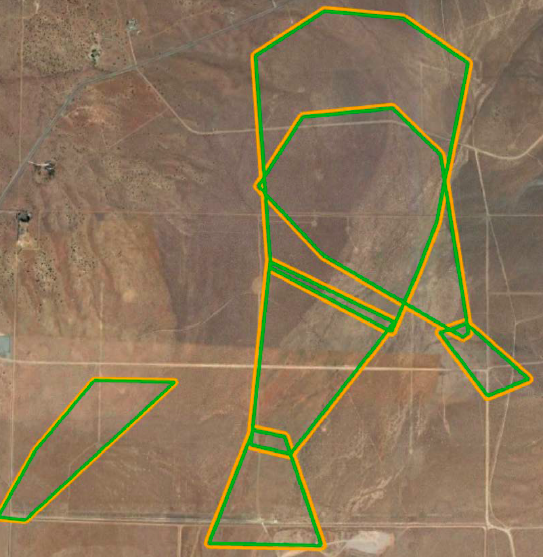
\includegraphics[height=0.45\textwidth]{img/strategic-deconfliction.png}
      \end{column}
   \end{columns}
\end{frame}

\begin{frame}
   \frametitle{Deconfliction}
   \framesubtitle{Tactical / Dynamic Reroute}
   \begin{columns}[t]
      \begin{column}{0.5\textwidth}
         Actor: UAS/Pilot/Operator \\
         Stage: During-flight \\
         APIs: UAS/Pilot $\leftrightarrow$ UTM; UTM $\leftrightarrow$ UTM; UTM $\leftrightarrow$ CAA \\
         Objective: Minimize the likelihood of airborne conflicts and maximize the likelihood of conforming to airspace restrictions and maintaining mission objectives. \\
         Operator Use: The directive guidance could be delivered to the UAS Operator or UAS depending on the mode of operation (e.g. pilot on-the-loop). Dynamic re-routing is an advanced service and relies on several other services.
      \end{column}
      \begin{column}{0.5\textwidth}
         Output: Directive guidance to resolve conflicts, remain clear or flight restricted areas, return to mission to support more automated UAS capabilities.
         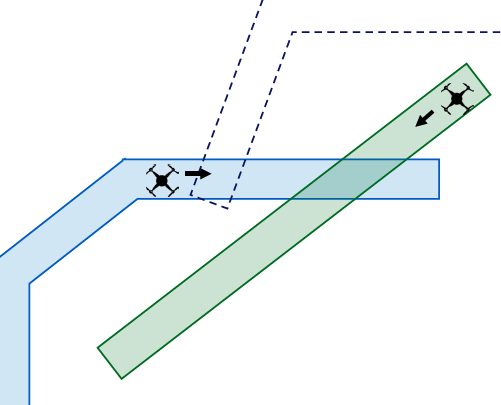
\includegraphics[height=0.45\textwidth]{img/dynamic-rerouting.png}

      \end{column}
   \end{columns}
\end{frame}

%------------------------------------------------

\section{Standardisation}
\subsection{Efforts}
\begin{frame}[fragile] % Need to use the fragile option when verbatim is used in the slide
   \frametitle{Standardisaton}
   \framesubtitle{Efforts}
   India and regulatory changes
   \begin{block}{NPNT}
      Improving standardisation and documentation
   \end{block}

   \begin{block}{DigitalSky\texttrademark}
      Recommendations for improvements and features
   \end{block}

\end{frame}

%------------------------------------------------

\subsection{Challenges}
\begin{frame}[fragile] % Need to use the fragile option when verbatim is used in the slide
   \frametitle{Standardisaton}
   \framesubtitle{Challenges}
   \begin{columns}[t]
      \column{.45\textwidth} % column designated by a command
      \begin{itemize}
         \item Rapidly evolving technology
            \begin{itemize}
               \item UAS internals
               \item Reliable Mobile Connectivity Infrastructure
               \item New commercial applications
            \end{itemize}
         \item Industry consensus difficult to achieve
            \begin{itemize}
                  \item Too many stakeholders
                  \item Diverse industries
            \end{itemize}
      \end{itemize}
      \column{.45\textwidth} % column designated by a command
      \begin{itemize}
         \item India still catching up on regulatory changes in EU/US, etc.
            \begin{itemize}
               \item Separation standards
               \item Remote Identification and tracking
            \end{itemize}
         \item Chicken before egg: Regulatory effort underway before industry has reached scale
      \end{itemize}
   \end{columns}
\end{frame}

%------------------------------------------------

\begin{frame}[fragile] % Need to use the fragile option when verbatim is used in the slide
   \frametitle{Standardisaton}
   \framesubtitle{Challenges}
   \begin{columns}[t]
      \column{.45\textwidth} % column designated by a command
      \begin{itemize}
         \item No concerted effort on standardising the way operational practices or risk assessments are evaluated by regulatory bodies
      \end{itemize}
   \end{columns}
\end{frame}

%------------------------------------------------

\begin{frame}[fragile] % Need to use the fragile option when verbatim is used in the slide
   \frametitle{Standardisaton}
   \framesubtitle{Future Work}
   \begin{columns}[t]
      \column{.45\textwidth} % column designated by a command
      \begin{itemize}
         \item Drone Swarms
         \item Drone Ports
         \item Drone Corridors
      \end{itemize}
      \column{.45\textwidth} % column designated by a command
      \begin{itemize}
         \item Interaction with Manned ATC
         \item Counter-UAS
         \item Emergency Management
      \end{itemize}
   \end{columns}
\end{frame}

%------------------------------------------------

\begin{frame}[t, allowframebreaks]
   \frametitle{References}
   % \bibliographystyle{plain}
   {\footnotesize
   \bibliographystyle{IEEEtran}
   \setcitestyle{square,numbers}

   \bibliography{../../research/Bibliography}
   }
\end{frame}

%------------------------------------------------

\begin{frame}
   \Huge{\centerline{The End}}
\end{frame}

%----------------------------------------------------------------------------------------

\end{document}
